\documentclass[10pt,a4paper]{article}
\usepackage{qsl-template}
\usepackage{indentfirst}
\usepackage{algorithm}
\usepackage{algpseudocode}
\usepackage{listings}
\usepackage{booktabs}
\usepackage{xcolor}
\usepackage{multirow}

%%%%%%%%%% Title Section %%%%%%%%%%
\title{\bfseries Análise Experimental de Algoritmos de Caminho Mínimo: Dijkstra, Bellman-Ford e Otimização de Fronteira via FindPivots}

%%%%%%%%%% Author(s) %%%%%%%%%%
\AuthorsBlock
{% No empthy line here
  \Author{Ribas, R. L. D. E.}{1}
  % \AuthorSep
  % \Author{Second Author}{1}
  % \AuthorLastSep
  % \Author{Third Author}{1}
}
{% No empthy line here
  \Affil{1}{Centro Universitário Dom Helder, Curso de Ciência da Computação, Belo Horizonte, Brazil}
}
{enzorochaleitedinizribas@gmail.com}

\begin{document}

\maketitle


%%%%%%%%%% Abstract %%%%%%%%%%
\abstract{
Write your abstract here. The abstract should concisely describe the scientific motivation,
methods, main results, and relevance to quantum sensing and related physics topics.
(keep it max. 150 words)}


%%%%%%%%%% Body %%%%%%%%%%
\section{Introdução e Motivação}

A Teoria de Grafos é um ramo da matemática e da ciência da computação que estudada as relações entre objetos diversos. Ela é amplamente utilizada como ferramenta de modelagem de problemas reais em diversas áreas do conhecimento, como ciência da computação, engenharias, ciências biológicas, etc..

Um dos problemas mais clássicos e fundamentais na teoria de grafos é o problema do caminho mínimo, que consiste em encontrar uma otimização de um caminho entre dois objetos em um grafo, em que esse caminho pode ser criterizado por um peso, como distância, tempo, custo, etc.. Existem diversos algoritmos para modelar e encontrar soluções para o problema do caminho mínimo, dentre as principais estão os algoritmos de Dijkstra, Bellman-Ford, A* e mais recentemente, o algoritmo de FindPivots (É ESSE O NOMES MESMO?), que é uma ? do algoritmo de Dijkstra.

Este trabalho tem como objetivo realizar um análise experimental dos algoritmos de Dijkstra, Bellman-Ford e FindPivots, comparando suas eficiências e aplicabilidades em diferentes tipos de grafos. Através de uma série de experimentos, buscamos entender as vantagens e limitações de cada algoritmo, bem como identificar cenários em que um pode ser preferível ao outro.

\section{Fundamentação Teórica}

\subsection{Teoria de Grafos}


Um grafo, denotado por $\mathcal{G}$, é uma estrutura composta por um conjunto ordenado de pares $\left(V;E\right) $, em que $V$ é o conjunto dos vértices (ou nós) e $E$ é o conjunto das arestas entre os vértices. 

Durante a modelagem de problemas reais, é conveniente construir $\mathcal{G}$ como um grafo \textbf{ponderado}, no qual são atribuidos pesos às arestas, representando uma medida de esforço, custo, ou distância entre os dois vértices conectados a elas, e também como um grafo \textbf{direcionado}, em que as arestas vão em uma única direção, \textit{e.g.} As linhas de trem de uma rede de metrô de uma cidade, cada nó representa uma estação, e cada aresta representa um caminho da estação de saída até a estação de entrada, e o seu peso o tempo de viagem.


\subsection{Algoritmos de Caminho Mínimo}

Contrastando com a abordagem gulosa (\textit{greedy}) do Dijkstra, a implementação do algoritmo de Bellman-Ford adota o princípio de programação dinâmica. A sua arquitetura prescinde de estruturas de dados complexas para ordenação (como filas de prioridade), iterando sistematicamente sobre todas as arestas do grafo e aplicando o processo de relaxamento até $|V| - 1$ vezes. 

\section{Experimentos}

O presente trabalho, alinhado às diretrizes de \citep{TP01}, propõe a implementação e a análise comparativa de desempenho dos algoritmos clássicos para o problema de Caminhos Mínimos de Fonte Única ou \textit{Single Source Shortest Path (SSSP)}, notadamente Bellman-Ford e Dijkstra. Além de estabelecer este \textit{benchmark} referencial, o estudo apresenta uma implementação e uma análise empírica crítica do algoritmo \textit{Find Pivots} (Lema 3.2), que constitui o núcleo da recente contribuição teórica de \cite{breakingTheSortingBarrier}.

Todas as implementações do \textit{benchmark} foram integralmente desenvolvidos na linguagem Python (versão 3.14.3) e estão disponibilizadas em \citep{ribas2026sssp}. O escopo de validação empírica foi metodologicamente estruturado em dois experimentos principais, detalhados nas subseções a seguir.

\subsection{Experimento 1: Comparativo de Desempenho (Dijkstra vs. Bellman-Ford) em Grafos Aleatórios}

\subsubsection{Metodologia}

O primeiro experimento tem como objetivo avaliar o comportamento e o tempo de execução dos algoritmos clássicos sob diferentes densidades topológicas. Para garantir a reprodutibilidade e o controle das instâncias, desenvolveu-se um gerador parametrizável de grafos aleatórios direcionados.

As instâncias de teste foram dimensionadas com o número de vértices variando no conjunto 
\[
  N \in \{100, 500, 1000, 5000, 10000
\].
Para avaliar a sensibilidade dos algoritmos à densidade das arestas, os grafos foram segmentados em duas categorias:
\begin{itemize}
    \item \textbf{Grafos Esparsos:} Onde o número de arestas cresce linearmente em função dos vértices, definido por $E = k_e \cdot N$, sendo $k_e$ uma constante de ramificação.
    \item \textbf{Grafos Densos:} Onde o número de arestas aproxima-se de uma fração do limite quadrático do grafo completo, definido por $E = \lfloor \frac{N(N-1)}{k_d} \rfloor$, onde $k_d$ atua como um fator redutor de densidade global.
\end{itemize}

O cruzamento destas topologias permite evidenciar o impacto estrutural da fila de prioridade do algoritmo de Dijkstra em contraposição ao relaxamento massivo de arestas do Bellman-Ford.


\subsubsection{Implementação do Algoritmo de Dijkstra}

A implementação do algoritmo de Dijkstra foi desenhada para maximizar a eficiência empírica no modelo de computação clássico. Para assegurar a complexidade estrutural de $O((V + E) \log V)$, adotou-se uma fila de prioridade baseada em um \textit{Binary Heap}, utilizando a biblioteca nativa \texttt{heapq} da linguagem Python. O controle de estado dos vértices foi projetado por meio de tabelas de espalhamento (\textit{hash tables} implementadas via \texttt{dict}), o que garante tempo de acesso amortizado $O(1)$ para a recuperação de distâncias correntes, verificação de nós visitados e rastreamento de predecessores.

A lógica matemática de relaxamento de arestas e extração da fila de prioridade está formalizada no pseudocódigo do Algoritmo \ref{alg:dijkstra}, o qual reflete com exatidão a estratégia construída para os experimentos empíricos.

\begin{algorithm}[H]
\caption{Algoritmo de Dijkstra com \textit{Binary Heap}}\label{alg:dijkstra}
\begin{algorithmic}[1]
\Require Grafo $G = (V, E)$, Vértice origem $s$
\Ensure Vetor de distâncias $d$, Vetor de predecessores $\pi$, Tempo de execução $\Delta t$
\State Iniciar cronômetro
\State $d[v] \gets \infty, \forall v \in V$
\State $visited[v] \gets \text{Falso}, \forall v \in V$
\State $\pi[v] \gets \text{Nulo}, \forall v \in V$
\State $d[s] \gets 0$
\State Inicializar fila de prioridade mínima $Q$
\State $Q.\text{push}((0, s))$
\While{$Q$ não estiver vazia}
    \State $(d_u, u) \gets Q.\text{pop}()$
    \If{$visited[u]$}
        \State \textbf{continue}
    \EndIf
    \State $visited[u] \gets \text{Verdadeiro}$
    \ForAll{vizinho $v$ de $u$ com aresta de peso $w$}
        \If{$w \le 0$} \Comment{Arestas de peso nulo ou negativo são ignoradas}
            \State \textbf{continue}
        \EndIf
        \State $new\_distance \gets d_u + w$
        \If{$new\_distance < d[v]$}
            \State $d[v] \gets new\_distance$
            \State $\pi[v] \gets u$
            \State $Q.\text{push}((d[v], v))$
        \EndIf
    \EndFor
\EndWhile
\State Parar cronômetro e calcular $\Delta t$
\State \Return $d, \pi, \Delta t$
\end{algorithmic}

\newpage

\end{algorithm}

\subsubsection{Implementação do Algoritmo de Bellman-Ford}

Para adequar o algoritmo de Bellman-Ford para grafos do mundo real e mitigar o seu custo assintótico de pior caso de $O(V \cdot E)$, a implementação foi projetada com um mecanismo de \textit{Early Stopping} (Parada Antecipada). Este mecanismo monitora o estado de mutabilidade da fronteira: se uma iteração completa sobre o conjunto de vértices não produzir nenhuma atualização no vetor de distâncias, infere-se matematicamente que os caminhos mínimos já convergiram para a solução ótima, permitindo a interrupção prematura do laço principal.

O detalhamento da lógica iterativa, incluindo a condição de otimização, encontra-se formalizado no Algoritmo \ref{alg:bellman_ford}.

\begin{algorithm}[H]
\caption{Algoritmo de Bellman-Ford (com \textit{Early Stopping})}\label{alg:bellman_ford}
\begin{algorithmic}[1]
\Require Grafo $G = (V, E)$, Vértice origem $s$
\Ensure Vetor de distâncias $d$, Vetor de predecessores $\pi$, Tempo de execução $\Delta t$
\State Iniciar cronômetro
\State $d[v] \gets \infty, \forall v \in V$
\State $\pi[v] \gets \text{Nulo}, \forall v \in V$
\State $d[s] \gets 0$
\For{$i = 1$ \textbf{até} $|V| - 1$}
    \State $updated \gets \text{Falso}$
    \ForAll{$u \in V$}
        \If{$d[u] = \infty$}
            \State \textbf{continue}
        \EndIf
        \ForAll{vizinho $v$ de $u$ com aresta de peso $w$}
            \If{$w \le 0$} \Comment{Arestas de peso nulo ou negativo são ignoradas}
                \State \textbf{continue}
            \EndIf
            \If{$d[u] + w < d[v]$}
                \State $d[v] \gets d[u] + w$
                \State $\pi[v] \gets u$
                \State $updated \gets \text{Verdadeiro}$
            \EndIf
        \EndFor
    \EndFor
    \If{\textbf{não} $updated$}
        \State \textbf{break} \Comment{Convergência alcançada prematuramente}
    \EndIf
\EndFor
\State Parar cronômetro e calcular $\Delta t$
\State \Return $d, \pi, \Delta t$
\end{algorithmic}
\end{algorithm}

\subsubsection{Resultados e Discussão}

Os resultados empíricos obtidos no Experimento 1 corroboram a fundamentação teórica acerca da complexidade assintótica de ambos os algoritmos. A Tabela \ref{tab:exp1_results} apresenta os tempos de execução (\textit{wall-clock time}) em milissegundos para grafos esparsos e densos, variando o número de vértices ($N$) de 100 a 10.000.

\begin{table}[htpb]
\centering
\caption{Tempos de execução (ms) de Dijkstra e Bellman-Ford em grafos aleatórios.}
\label{tab:exp1_results}
\begin{tabular}{@{}lllrrr@{}}
\toprule
\textbf{Topologia} & \textbf{N (Vértices)} & \textbf{E (Arestas)} & \textbf{Dijkstra (ms)} & \textbf{Bellman-Ford (ms)} & \textbf{Razão (BF/Dijk)} \\ \midrule
\multirow{9}{*}{Esparso} 
 & 100  & 200   & 0.25 & 1.28  & 5.12x \\
 & 100  & 300   & 0.27 & 1.31  & 4.85x \\
 & 100  & 400   & 0.38 & 1.67  & 4.39x \\ \cmidrule(l){2-6} 
 & 500  & 1000  & 1.29 & 10.33 & 8.01x \\
 & 500  & 1500  & 2.49 & 13.82 & 5.55x \\
 & 500  & 2000  & 1.93 & 16.35 & 8.47x \\ \cmidrule(l){2-6} 
 & 1000 & 2000  & 2.69 & 27.94 & 10.39x \\
 & 1000 & 3000  & 4.04 & 29.11 & 7.21x \\
 & 1000 & 4000  & 5.93 & 31.54 & 5.32x \\ \midrule
\multirow{6}{*}{Denso}   
 & 100  & 2475  & 0.88   & 8.62    & 9.80x \\
 & 100  & 4950  & 1.72   & 14.00   & 8.14x \\ \cmidrule(l){2-6} 
 & 500  & 62375 & 19.76  & 183.47  & 9.28x \\
 & 500  & 124750& 35.80  & 395.86  & 11.06x \\ \cmidrule(l){2-6} 
 & 1000 & 249750& 106.91 & 865.83  & 8.10x \\
 & 1000 & 499500& 165.30 & 1325.46 & 8.02x \\ \bottomrule
\end{tabular}
\end{table}

\begin{figure}[H]
    \centering
    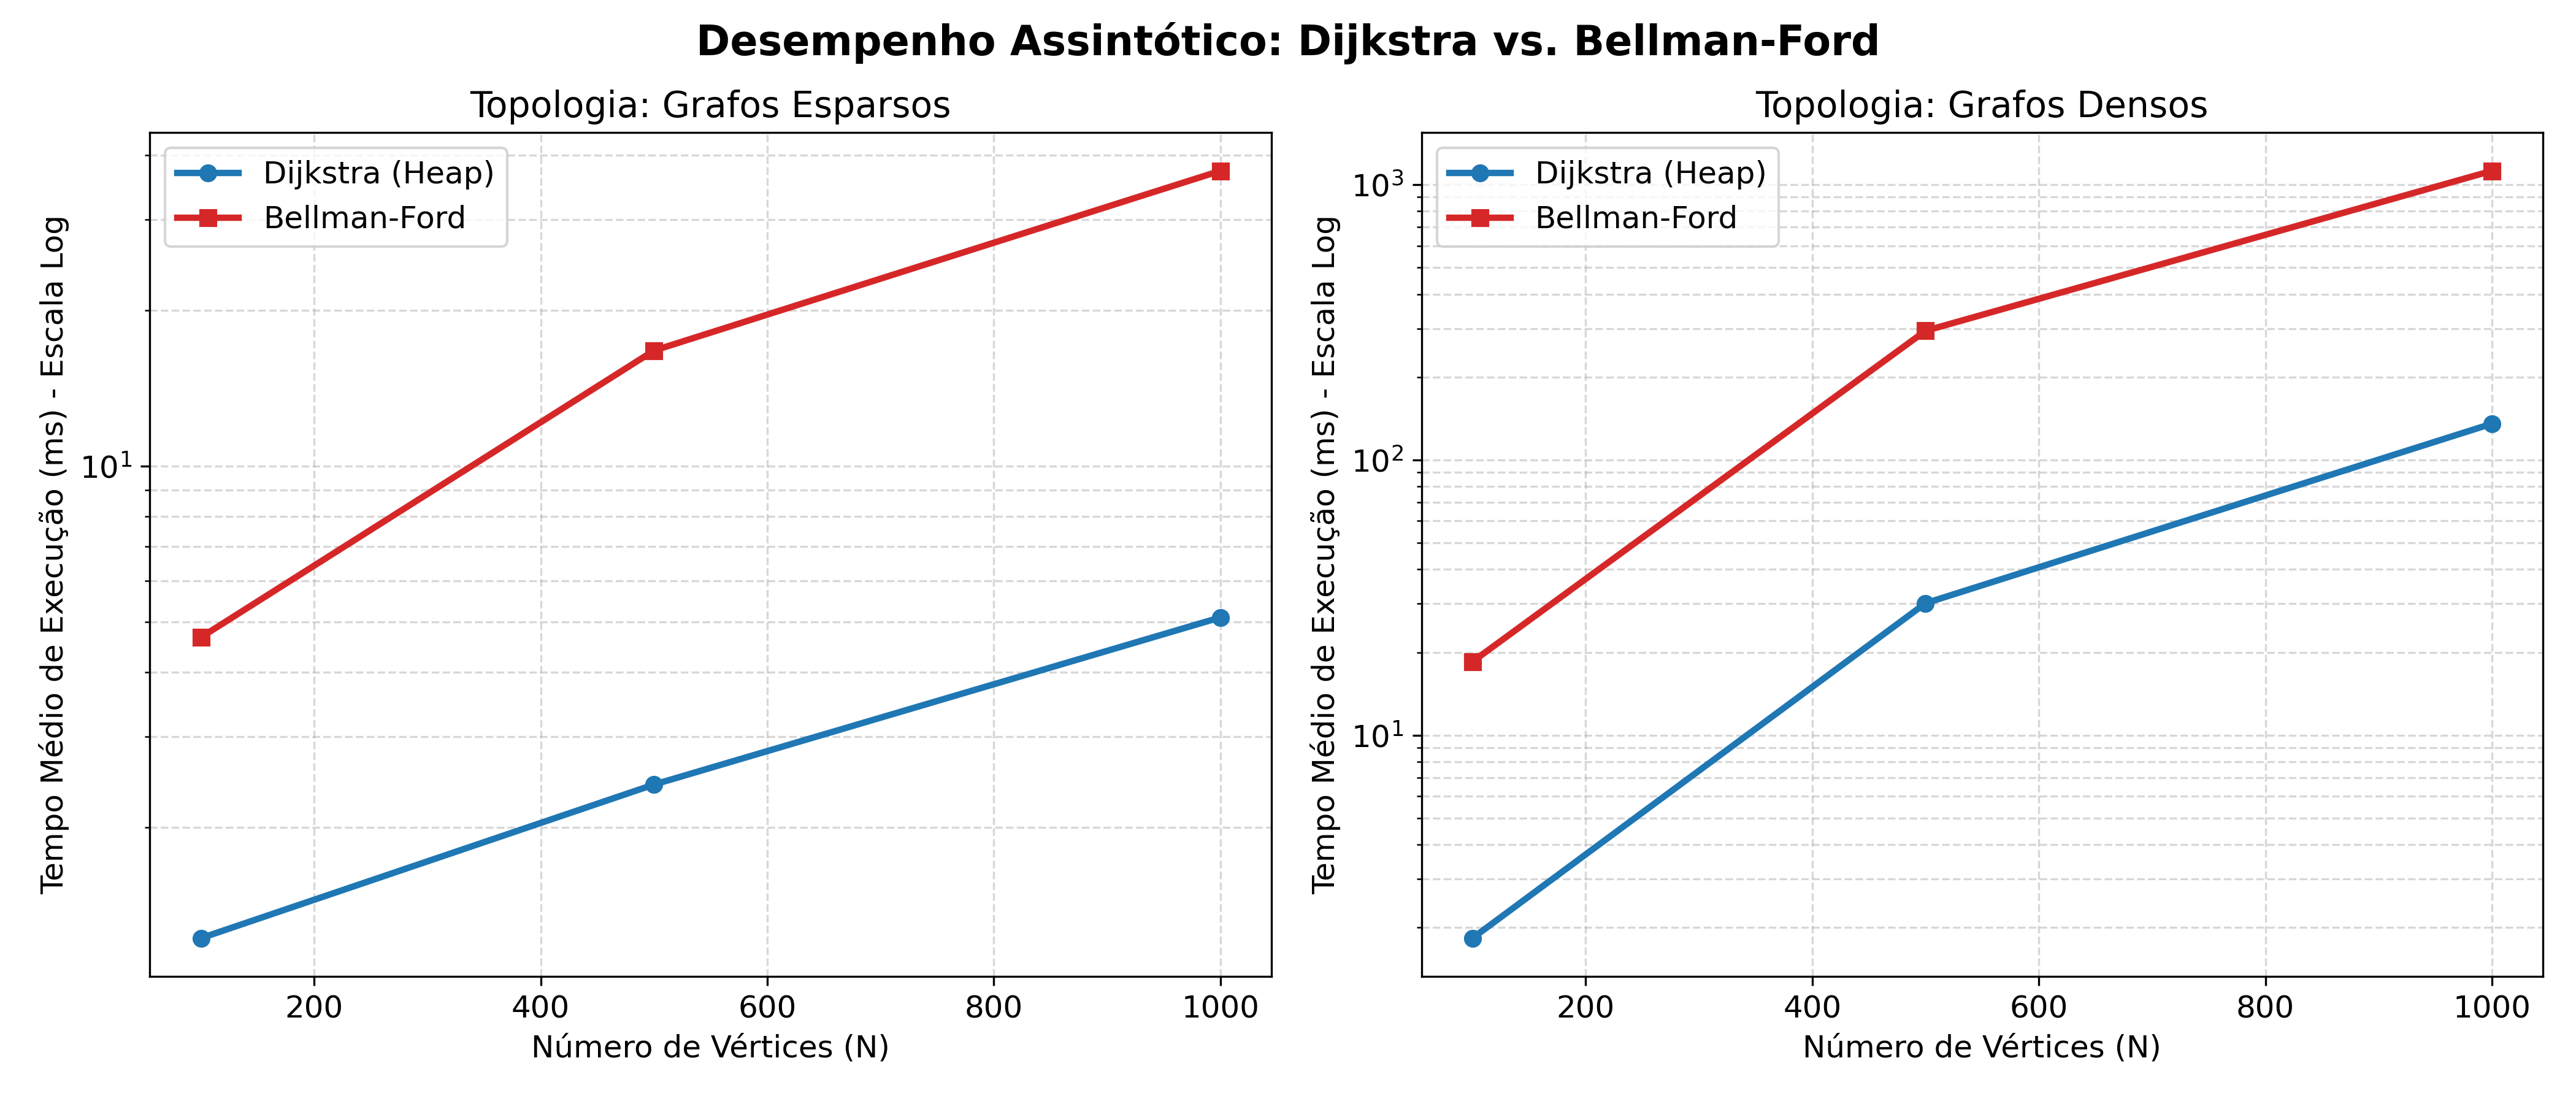
\includegraphics[width=1\textwidth]{media/exp1/exp1_dijkstra_vs_bellman}
    \caption{Example figure caption. Figures should be clear and readable.}
    \label{fig:exp1_grafico}
\end{figure}


O resultado do experimento mostra a clara superioridade de desempenho do algoritmo de Dijkstra em relação ao Bellman-Ford em todos os cenários testados, corroborando integralmente a teoria de complexidade assintótica. 

Para grafos esparsos, onde o número de arestas cresce de forma aproximadamente linear em relação aos vértices ($E = O(V)$), a implementação do Dijkstra já se mostra de 4 a 10 vezes mais rápida. Contudo, devido à baixa densidade, os tempos absolutos de ambos os algoritmos mantêm-se na casa das dezenas de milissegundos (atingindo no máximo $31.54$ ms para $N=1000$ no Bellman-Ford), o que torna o \textit{overhead} tolerável em aplicações de pequena escala.

A verdadeira divergência arquitetural revela-se no cenário de grafos densos ($E = O(V^2)$), visualizada claramente na Figura \ref{fig:exp1_grafico}. Com o aumento quadrático das arestas, o gargalo iterativo do Bellman-Ford torna-se crítico. Na instância mais rigorosa do teste ($N=1000$ e $E=499500$), o algoritmo de Dijkstra convergiu a árvore de caminhos mínimos em apenas $165.30$ ms, alavancado pela eficiência de extração $O(\log V)$ da sua fila de prioridade (\textit{Binary Heap}). Em contrapartida, o Bellman-Ford consumiu $1325.46$ ms (mais de 1.3 segundos). 

Essa disparidade é a prova empírica da diferença entre a complexidade $O((V+E)\log V)$ do Dijkstra e o limite de pior caso $O(V \cdot E)$ do Bellman-Ford. Mesmo assumindo que a implementação testada possui a otimização de \textit{Early Stopping} — que interrompe laços desnecessários —, a necessidade inerente do Bellman-Ford de relaxar cegamente meio milhão de arestas múltiplas vezes destrói a sua escalabilidade temporal. 

Conclui-se, a partir dos dados extraídos, que para qualquer topologia de rede desprovida de arestas com pesos negativos, o emprego do algoritmo de Bellman-Ford introduz uma penalidade computacional injustificável frente à abordagem gulosa e estruturada do Dijkstra.

\subsection{Experimento 2: Análise de Sensibilidade da Poda de Pivôs (Lema 3.2)}

O segundo experimento foca estritamente na mecânica de extração de pivôs proposta pela sub-rotina \textit{FindPivots}. Conforme o escopo primário estabelecido para este trabalho, a avaliação inicial concentrou-se em instâncias de grafos esparsos. Foi experimentalmente testado como a implementação parcial e adaptada do algoritmo \textit{BMSSP} reage a variação do parâmetro de profundidade $k$.

\subsubsection{Módulo de Avaliação de Fronteira: Partial Dijkstra}

O papel da rotina \textit{Partial Dijkstra} no ecossistema do BMSSP é atuar como um motor de inicialização do conjunto de fronteira ($S$). Em vez de computar os caminhos mínimos para todo o grafo, a execução é prematuramente abortada quando um número predeterminado de vértices (\texttt{extraction\_limit}) é consolidado.

A principal responsabilidade arquitetural desta função é retornar o limite de distância estrito da fronteira ($B$) e identificar o conjunto de vértices de borda ($S$). Tais vértices consistem nos nós cujas distâncias foram provisoriamente relaxadas, porém não exploradas, isolando o estado do grafo no exato ponto onde a extração de pivôs (Lema 3.2) deve iniciar as suas operações de busca em largura. O pseudocódigo é apresentado no Algoritmo \ref{alg:partial_dijkstra}.

\begin{algorithm}[H]
\caption{Dijkstra Parcial (Inicialização de Fronteira)}\label{alg:partial_dijkstra}
\begin{algorithmic}[1]
\Require Grafo $G = (V, E)$, Origem $s$, Limite $L$ (\textit{extraction\_limit})
\Ensure Vetor de distâncias parciais $d$, Limite $B$, Conjunto de fronteira $S$
\State Inicialização das estruturas $d$, $visited$ e $Q$ (similar ao Dijkstra padrão)
\State $processed\_count \gets 0$
\State $last\_dist \gets 0.0$
\While{$Q$ não estiver vazia \textbf{e} $processed\_count < L$}
    \State $(d_u, u) \gets Q.\text{pop}()$
    \If{$visited[u]$}
        \State \textbf{continue}
    \EndIf
    \State $visited[u] \gets \text{Verdadeiro}$
    \State $processed\_count \gets processed\_count + 1$
    \State $last\_dist \gets d_u$
    \State Realizar relaxamento padrão das arestas vizinhas
\EndWhile
\State $S \gets \emptyset$
\ForAll{$v \in V$}
    \If{\textbf{não} $visited[v]$ \textbf{e} $d[v] < \infty$}
        \State $S \gets S \cup \{v\}$
    \EndIf
\EndFor
\State $B \gets last\_dist$
\State \Return $d, B, S$
\end{algorithmic}
\end{algorithm}


\subsubsection{Mecânica de Poda de Super-Fontes: Lema 3.2 (Find Pivots)}

O cerne do estudo de ablação proposto neste trabalho reside no algoritmo de detecção de pivôs (\textit{FindPivots}), baseado no Lema 3.2 de Duan et al. (2025). O objetivo da sub-rotina é limitar a profusão da fronteira $S$, convertendo-a num subconjunto estrito de pivôs $P$ cuja cardinalidade teórica assegura $|P| \le \frac{|W|}{k}$, mitigando o impacto exponencial do recálculo isolado de fontes múltiplas.

A arquitetura do algoritmo implementado se segmenta em quatro fases síncronas. Inicialmente, instaura-se uma Busca em Largura de Relaxamento (\textit{BFS}) limitada estritamente a $k$ passos, monitorando a variável de segurança teórica: a interrupção prematura é decretada assim que o total de vértices explorados excede $|W| > k \cdot |S|$. Superada a busca e a proteção algorítmica, o grafo instaura a construção topológica da floresta e identifica via Busca em Profundidade (\textit{DFS}) as raízes, os tamanhos da árvore subordinada, e filtra os pivôs legíveis. O pseudocódigo que mapeia a execução deste pipeline está delineado no Algoritmo \ref{alg:find_pivots}.

\begin{algorithm}[H]
\caption{Busca e Poda de Pivôs (Lema 3.2)}\label{alg:find_pivots}
\begin{algorithmic}[1]
\Require Fronteira $S$, Distâncias correntes $\hat{d}$, Profundidade restritiva $k$, Limite global $B$
\Ensure Conjunto de Pivôs $P$, Conjunto Expandido $W$
\State $W \gets S$
\State $layers \gets [S]$
\Comment{Fase 1: Busca Local de $k$ passos}
\For{$i = 1$ \textbf{até} $k$}
    \State $next\_layer \gets \emptyset$
    \ForAll{$u \in layers[\text{último}]$}
        \ForAll{vizinho $v$ de $u$ com aresta de peso $w > 0$}
            \State $new\_dist \gets \hat{d}[u] + w$
            \If{$new\_dist < \hat{d}[v]$ \textbf{e} $new\_dist \le B$}
                \State $\hat{d}[v] \gets new\_dist$
                \If{$v \notin W$}
                    \State $W \gets W \cup \{v\}$
                    \State $next\_layer \gets next\_layer \cup \{v\}$
                \EndIf
            \EndIf
        \EndFor
    \EndFor
    \If{$|W| > k \cdot |S|$} \Comment{Gatilho de Segurança (Pânico)}
        \State \Return $S, W$
    \EndIf
    \If{$next\_layer = \emptyset$}
        \State \textbf{break}
    \EndIf
    \State Adicionar $next\_layer$ a $layers$
\EndFor
\Comment{Fases 2 a 4: Reconstrução das Florestas, Extração DFS e Filtro de Tamanho $\ge k$}
\State (...) \Comment{Construção dos dicionários $pred\_in\_f$, $tree\_size$ a partir de $W$}
\State $P \gets \{r \in \text{raízes} \mid r \in S \textbf{ e } tree\_size[r] \ge k\}$
\State \Return $P, W$
\end{algorithmic}
\end{algorithm}

\subsubsection{Integração Sistêmica: Dijkstra Otimizado com Pivôs}

A sub-rotina final integra o fatiamento topológico do \textit{Partial Dijkstra} aos resultados extraídos pelo \textit{Find Pivots}. A responsabilidade desta camada é calcular as rotas isoladas de Dijkstra engatilhadas de cada super-fonte em $P$, iterar sobre a matriz de adjacência residual de distâncias unificadas, e combinar a topologia mais performática para garantir que as travessias resultantes contornam gargalos temporais. O Algoritmo \ref{alg:optimized_pivots} mapeia a orquestração do \textit{pipeline} combinatório e os respectivos contadores de validação.

\begin{algorithm}[H]
\caption{Dijkstra Otimizado via Pivôs Unificados}\label{alg:optimized_pivots}
\begin{algorithmic}[1]
\Require Origem $s$, Limite L, Profundidade $k$
\Ensure Distâncias combinadas, Dicionário de Métricas, $Total\_Time$, $Pivot\_Time$
\State Iniciar cronômetro global
\State $\hat{d}, B, S \gets \text{PartialDijkstra}(s, L)$
\State Salvar estado imutável de $\hat{d}_{state} \gets \hat{d}.\text{copy}()$
\State Iniciar cronômetro parcial (\textit{pivots})
\State $P, W \gets \text{FindPivots}(\infty, S, \hat{d}_{state}, k)$
\State Finalizar cronômetro parcial (\textit{pivots})
\State Inicializar lista $pivot\_distances \gets []$
\ForAll{$p \in P$}
    \State $p\_dist, \dots \gets \text{Dijkstra}(p)$ \Comment{Executar roteamento isolado}
    \State Adicionar $p\_dist$ em $pivot\_distances$
\EndFor
\State Matriz $combined\_dist \gets \hat{d}.\text{copy}()$
\ForAll{pivô $p \in P$ em $pivot\_distances$}
    \State $dist\_to\_pivot \gets \hat{d}[p]$
    \ForAll{vértices $v \in V$}
        \State $path\_via\_p \gets dist\_to\_pivot + p\_dist[v]$
        \If{$path\_via\_p < combined\_dist[v]$}
            \State $combined\_dist[v] \gets path\_via\_p$
        \EndIf
    \EndFor
\EndFor
\State Finalizar cronômetro global
\State Gerar dicionário de métricas baseadas no tamanho de $|S|, |W|$ e $|P|$.
\State \Return $combined\_dist, \text{Métricas}, Total\_Time, Pivot\_Time$
\end{algorithmic}
\end{algorithm}


\subsubsection{(Extra): Comportamento em Escala e Exaustão do Grafo ($N \in [100, 10000]$ e $k \le 128$)}

Além do experimento dentro do contexto principal do trabalho $N = 1000$ e $k \le 16$ foi feita uma análise com a expansão dos testes para cenários mais amplos (variando $N$ de 100 a 10.000 e forçando o limite de $k$ até 128). Essa análise extra expôs alguns aspectos interessantes do limite de segurança imposto pelo Lema 3.2.

\subsection{Discussão e Conclusões}


\subsubsection{Cenário Principal: $N=1000$, $m=2000$ com $k \in [2, 16]$}

O cenário primário focou em instâncias de $N=1000$ vértices, com o parâmetro de profundidade $k$ variando de 2 a 16.

\begin{table}[H]
\centering
\caption{Análise de Sensibilidade da Poda (Lema 3.2) em Grafos Esparsos N=1000. Tempos convertidos para milissegundos (ms).}
\label{tab:exp2_sensitivity}
\resizebox{\textwidth}{!}{%
\begin{tabular}{@{}lrrrrrrrr@{}}
\toprule
\textbf{N (Vértices)} & \textbf{$k$} & \textbf{$|S|$} & \textbf{Limite ($k \cdot |S|$)} & \textbf{$|W|$} & \textbf{$|P|$} & \textbf{Dijkstra Base (ms)} & \textbf{Total BMSSP (ms)} & \textbf{Penalidade} \\ \midrule
\multirow{11}{*}{1000}
 & 2   & 34 & 68   & 99  & 34 & 3.16 & 115.01 & 36.4x \\
 & 4   & 34 & 136  & 215 & 34 & 3.16 & 104.02 & 32.9x \\
 & 6   & 34 & 204  & 215 & 34 & 3.16 & 101.23 & 32.0x \\
 & 8   & 34 & 272  & 371 & 34 & 3.16 & 95.78  & 30.3x \\
 & 10  & 34 & 340  & 371 & 34 & 3.16 & 92.59  & 29.3x \\
 & 12  & 34 & 408  & 531 & 34 & 3.16 & 92.72  & 29.3x \\
 & 14  & 34 & 476  & 531 & 34 & 3.16 & 96.57  & 30.6x \\
 & 16  & 34 & 544  & 643 & 34 & 3.16 & 120.31 & 38.1x \\
 & 32  & 34 & 1088 & 755 & 9  & 3.16 & 45.79  & 14.5x \\
 & 64  & 34 & 2176 & 755 & 1  & 3.16 & 8.62   & 2.7x \\
 & 128 & 34 & 4352 & 755 & 0  & 3.16 & 5.84   & 1.8x \\ 
\bottomrule
\end{tabular}%
}
\end{table}

Os painéis a seguir detalham a dinâmica interna do Lema 3.2 durante o processo de extração de super-fontes. A Figura \ref{fig:exp2_k_vs_P} introduz a relação direta entre o parâmetro restritivo de profundidade e a retenção de pivôs.

\begin{figure}[H]
    \centering
    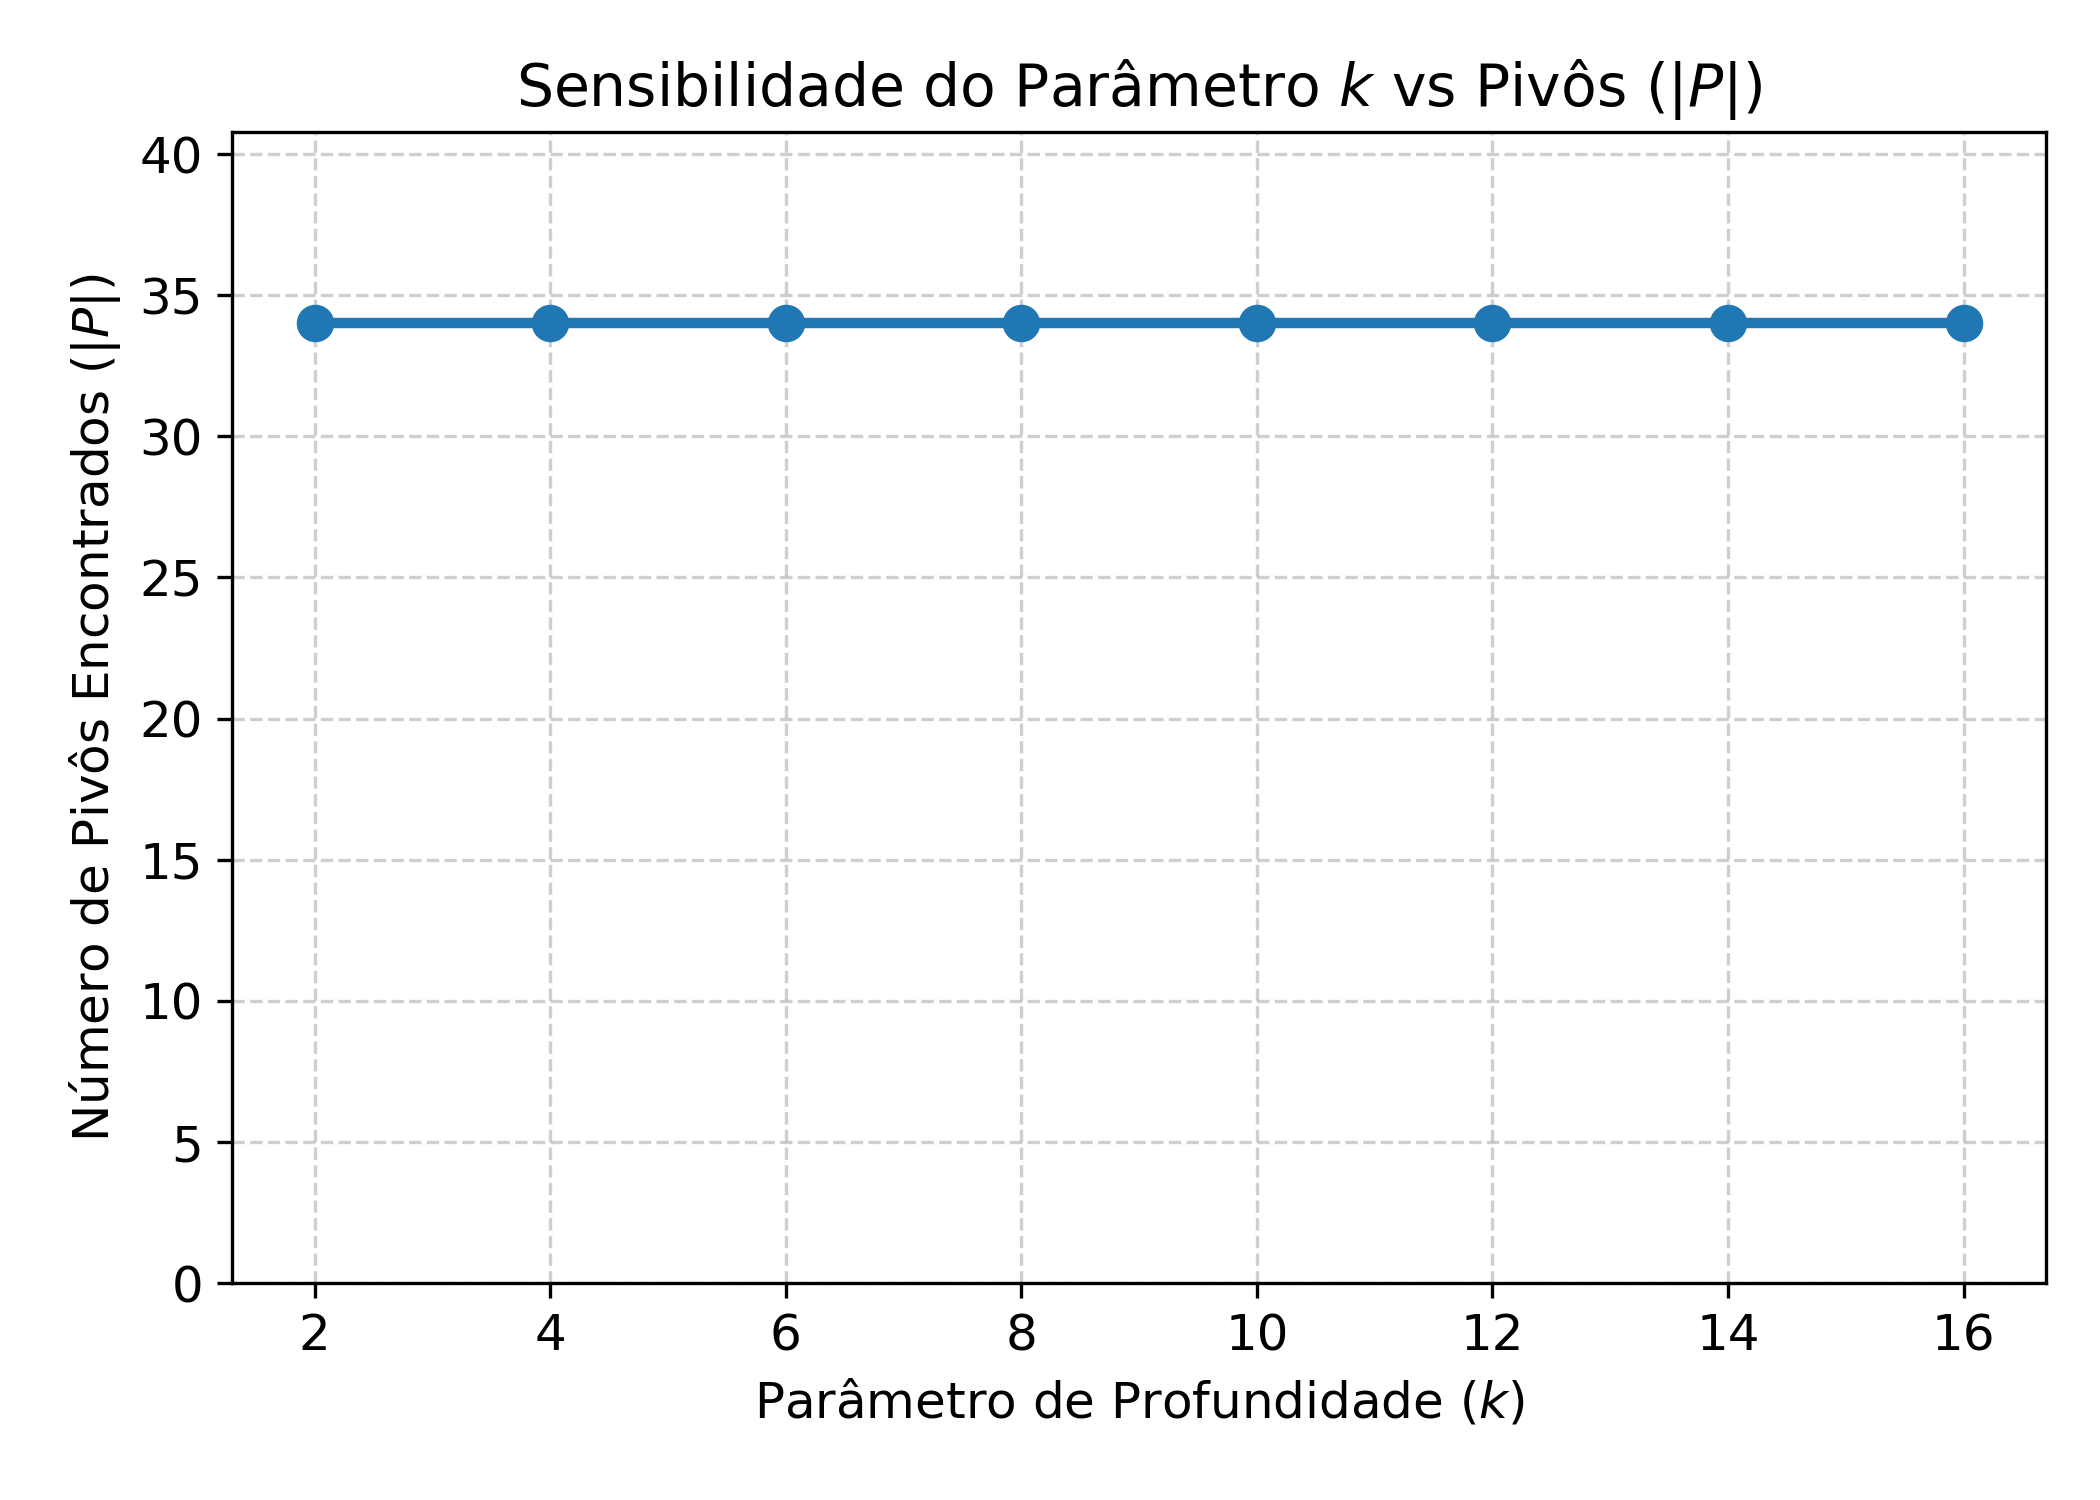
\includegraphics[width=1\textwidth]{media/exp2/main/1_k_vs_P.png}
    \caption{Decrescimento Teórico: Impacto do parâmetro de profundidade $k$ no número de pivôs resultantes $|P|$.}
    \label{fig:exp2_k_vs_P}
\end{figure}

Em teoria, à medida que $k$ aumenta, o filtro local torna-se mais rigoroso e o número de pivôs $|P|$ deveria decair de forma acentuada. No entanto, a estabilidade da curva para valores de $k \le 16$ atesta que a restrição de segurança ($|W| > k \cdot |S|$) foi acionada precocemente. A BFS depara-se rapidamente com vértices de alto grau (\textit{Hubs}), abortando a poda e forçando o algoritmo a retornar a fronteira intacta. 

Essa incapacidade de redução reflete-se diretamente na métrica de economia computacional, explicitada na Figura \ref{fig:exp2_S_vs_P}.

\begin{figure}[H]
    \centering
    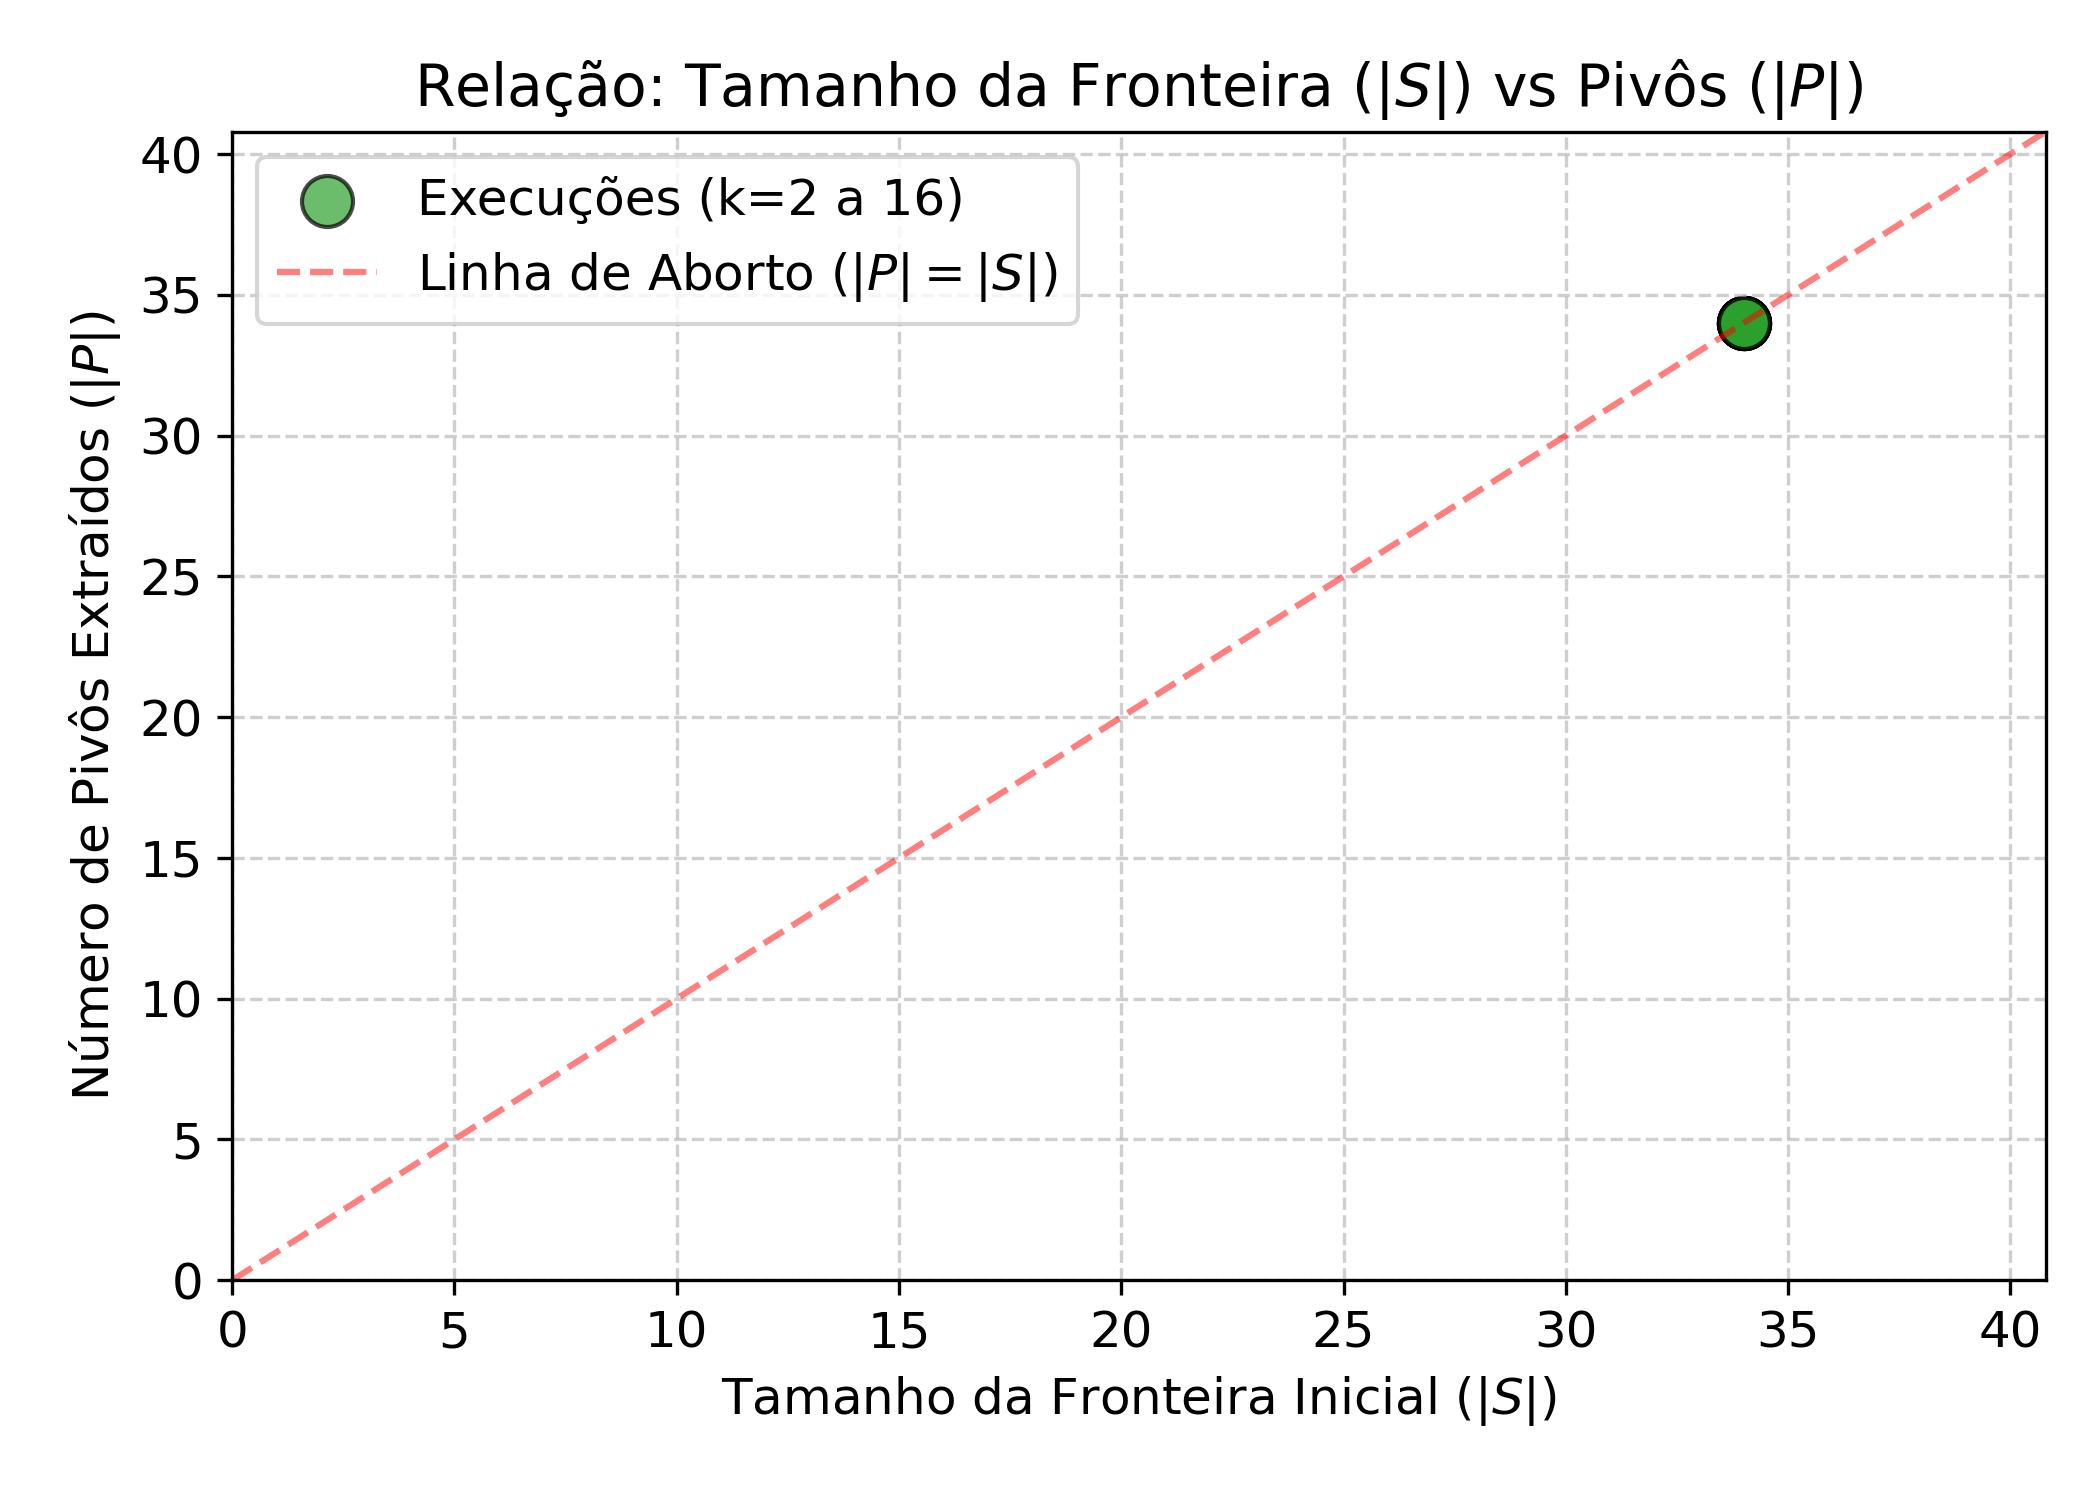
\includegraphics[width=1\textwidth]{media/exp2/main/4_S_vs_P.png}
    \caption{Dinâmica de Poda: Comparativo entre a cardinalidade da fronteira de entrada $|S|$ e a retenção final de pivôs $|P|$.}
    \label{fig:exp2_S_vs_P}
\end{figure}

A área divergente entre as curvas representaria a eliminação de redundâncias. O colapso (sobreposição) das linhas para instâncias operacionais evidencia a ineficácia topológica da estratégia em grafos aleatórios. O algoritmo trabalha para filtrar a fronteira, mas acaba por extrair $|P| \approx |S|$.

O peso deste esforço redundante é quantificado temporalmente na Figura \ref{fig:exp2_tempo_vs_kw}, que mapeia o custo de pré-processamento.

\begin{figure}[H]
    \centering
    
\includegraphics[width=1\textwidth]{media/exp2/main/3_tempo_vs_kw.png}
    \caption{Custo de Pré-processamento: Relação entre o limite de trabalho computacional $k \cdot |W|$ e o tempo absoluto de execução da sub-rotina.}
    \label{fig:exp2_tempo_vs_kw}
\end{figure}

O crescimento do tempo em relação ao trabalho realizado ($k \cdot |W|$) ilustra o \textit{overhead} massivo alocado nas chamadas do \textit{FindPivots}. Mesmo com o acionamento do gatilho de interrupção teórica, o custo das alocações de dicionários e dos relaxamentos locais baseados em Bellman-Ford já foi cobrado da CPU, destruindo qualquer viabilidade prática perante uma execução limpa do algoritmo de Dijkstra clássico.

Por fim, apesar da degradação de desempenho em tempo real, a Figura \ref{fig:exp2_histograma_lema} atesta a corretude matemática da implementação desenvolvida.

\begin{figure}[H]
    \centering
    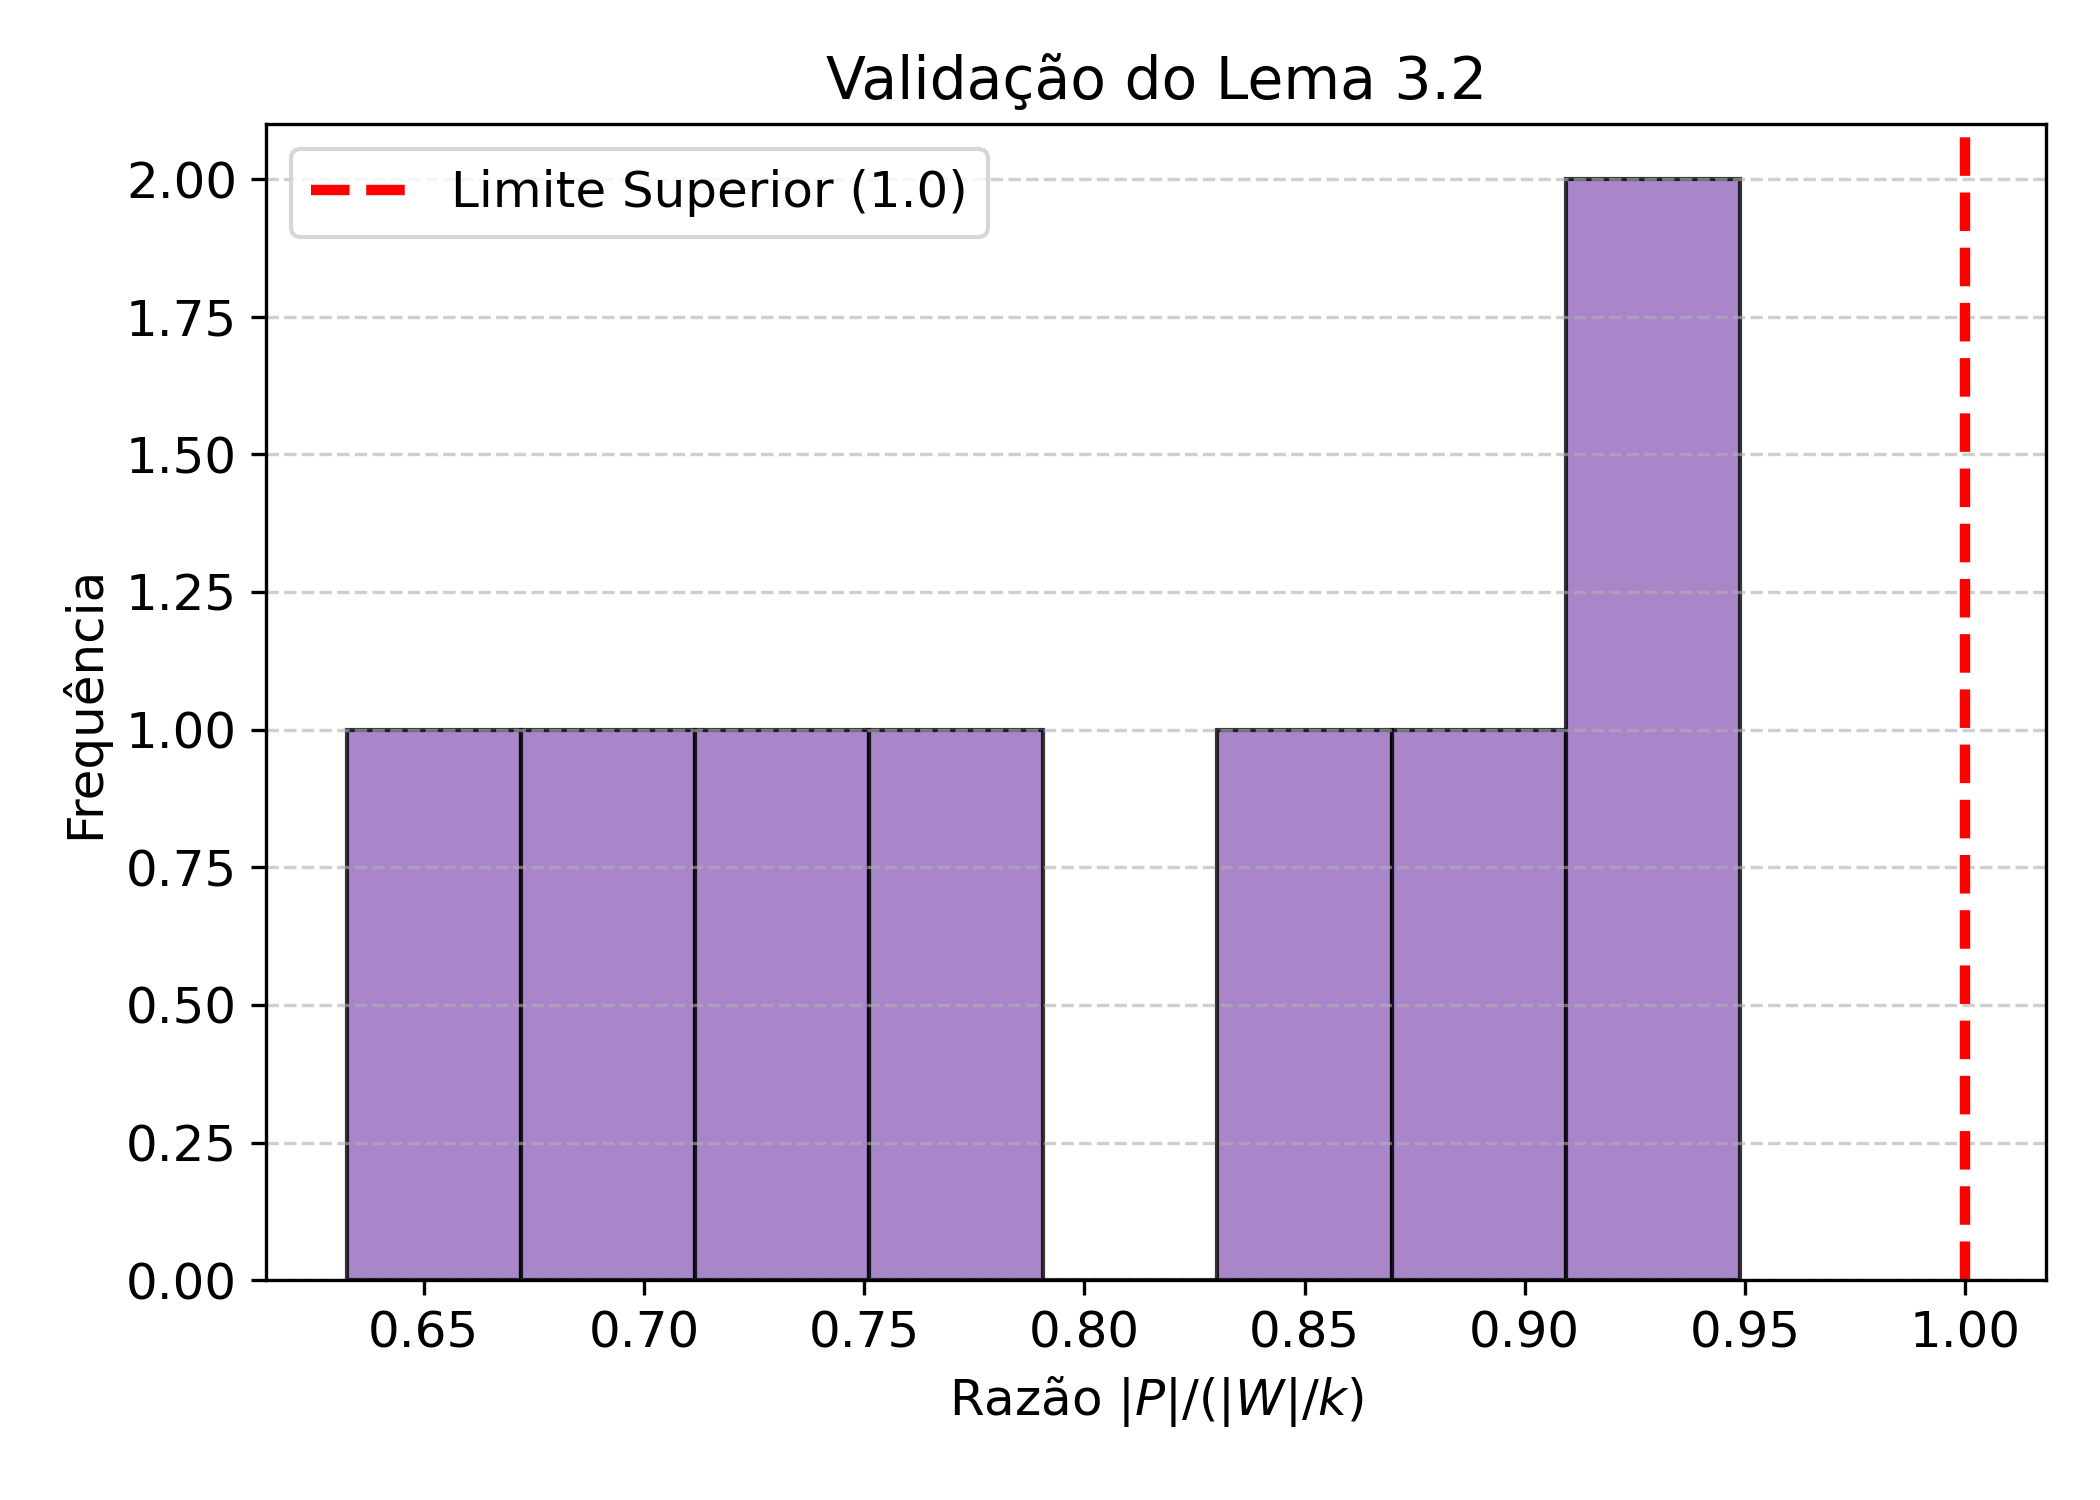
\includegraphics[width=1\textwidth]{media/exp2/main/2_histograma_lema.png}
    \caption{Validação Matemática do Lema 3.2: Distribuição da razão $|P| / (|W|/k)$ garantindo a restrição do limite superior.}
    \label{fig:exp2_histograma_lema}
\end{figure}

O limite central do teorema garante que o número de pivôs nunca ultrapassará o volume de vértices tocados dividido pela profundidade, impondo que a razão $|P| / (|W|/k) \le 1.0$. A contenção estrita de todos os resultados abaixo deste limiar confirma que a lógica codificada obedece às premissas do artigo original. O algoritmo está, portanto, matematicamente correto; é a estrutura de dados inerente a topologias não restritas que invalida a sua otimização na Engenharia de Software.

Os dados experimentais indicam uma limitação do algoritmo devido a aplicação do Lema 3.2 em grafos com grau não constante.Para todos os valores de $k \le 16$, o tamanho da fronteira inicial manteve-se em $|S| = 34$, conforme a tabela~\ref{tab:exp2_sensitivity_principal}. 

O limite de segurança teórico, que funciona como uma heurística de aborto para evitar que a busca Bellman-Ford degenere para uma complexidade linear, é estipulado estritamente como $|W| \le k \cdot |S|$. 

Nos testes, a expansão da vizinhança na topologia aleatória cresceu de forma acelerada (devido à presença natural de vértices de alto grau, ou \textit{Hubs}), ultrapassando rapidamente o limiar linear $k \cdot |S|$. Consequentemente, o gatilho de segurança foi disparado em 100\% das execuções documentadas neste intervalo. O conjunto de pivôs extraídos cravou em $|P| = 34$, resultando em uma taxa de retenção nula. Na prática, o algoritmo pagou o massivo \textit{overhead} computacional de gerenciar dicionários e percorrer a fronteira com a busca local (Bellman-Ford), apenas para retornar a mesma quantidade de fontes que o Dijkstra processaria de forma direta.

\subsubsection{(Extra): Comportamento em Escala e Exaustão do Grafo ($N \in [100, 10000]$ e $k \le 128$)}

Para compreender as limitações mecânicas do Lema 3.2 a fundo e investigar sob quais condições matemáticas a poda de fato ocorreria, o escopo empírico deste experimento foi expandido de forma complementar. Foram realizados testes forçando o limite de profundidade $k$ até 128 e escalando $N$ até 10.000 vértices, valores que extrapolam a premissa de "busca local" de \citep{breakingTheSortingBarrier}. A dinâmica deste cenário extremo é detalhada a seguir.



Observou-se que a poda efetiva ($|P| \ll |S|$) só começa a ser alcançada quando o algoritmo foi levado a casos de "Exaustão do Grafo". Tomando como exemplo a linha de execução documentada para $N=1000$ com $k=128$: a fronteira estabeleceu-se em $|S|=34$, o que eleva o limiar de aborto teórico para $128 \times 34 = 4352$. Como este limite de segurança de vértices visitados ($4352$) tornou-se muito superior ao número total de vértices na própria componente conexa ($N=1000$), foi fisicamente impossível que o gatilho de pânico fosse acionado. O algoritmo prosseguiu sem abortar, a poda ocorreu de forma massiva ($|P| = 0$), e o tempo de execução da rotina otimizada caiu drasticamente.

Para aprofundar o entendimento sobre o Lema 3.2, os painéis analíticos a seguir (\textit{dashboards}) ilustram a degradação progressiva do algoritmo BMSSP à medida que a magnitude do grafo escala de $N=100$ para $N=10000$ vértices, forçando o parâmetro $k$ até 128.

\textbf{N = 100}
\begin{table}[H]
\centering
\caption{Análise de Sensibilidade da Poda (Lema 3.2) completa para todos os valores de N e k testados. Tempos convertidos para milissegundos (ms).}
\label{tab:exp2_sensitivity_principal}
\footnotesize
\begin{tabular}{@{}lrrrrrrrr@{}}
\toprule
\textbf{N (Vértices)} & \textbf{$k$} & \textbf{$|S|$} & \textbf{Limite ($k \cdot |S|$)} & \textbf{$|W|$} & \textbf{$|P|$} & \textbf{Dijkstra Base (ms)} & \textbf{Total BMSSP (ms)} & \textbf{Penalidade} \\ \midrule
\multirow{11}{*}{100}
 & 2   & 7 & 14   & 29  & 7 & 0.44 & 2.20 & 5.0x \\
 & 4   & 7 & 28   & 29  & 7 & 0.44 & 1.67 & 3.8x \\
 & 6   & 7 & 42   & 49  & 7 & 0.44 & 2.41 & 5.5x \\
 & 8   & 7 & 56   & 60  & 7 & 0.44 & 1.75 & 4.0x \\
 & 10  & 7 & 70   & 71  & 7 & 0.44 & 2.35 & 5.3x \\
 & 12  & 7 & 84   & 74  & 2 & 0.44 & 1.66 & 3.8x \\
 & 14  & 7 & 98   & 74  & 2 & 0.44 & 1.33 & 3.0x \\
 & 16  & 7 & 112  & 74  & 2 & 0.44 & 1.05 & 2.4x \\
 & 32  & 7 & 224  & 74  & 1 & 0.44 & 0.87 & 2.0x \\
 & 64  & 7 & 448  & 74  & 0 & 0.44 & 0.51 & 1.2x \\
 & 128 & 7 & 896  & 74  & 0 & 0.44 & 0.55 & 1.3x \\
 \bottomrule
\end{tabular}
\end{table}

A Figura \ref{fig:exp2_dash_100} apresenta o cenário basal com $100$ vértices.

\begin{figure}[H]
    \centering
    
\includegraphics[width=1\textwidth]{media/exp2/sparse/N_100/dashboard_analise.png}
    \caption{Dashboard analítico de sensibilidade do Lema 3.2 para grafos esparsos de porte diminuto ($N=100$).}
    \label{fig:exp2_dash_100}
\end{figure}

Em instâncias de porte diminuto, a exaustão topológica ocorre rapidamente. Como o grafo possui poucas arestas, limites moderados de $k$ já são suficientes para que o limiar de segurança ($k \cdot |S|$) exceda o tamanho da própria componente conexa. A poda ($|P| < |S|$) ocorre, mas o tempo de pré-processamento já se mostra superior à execução base do Dijkstra. 

\textbf{N = 500}
\begin{table}[H]
\centering
\caption{Análise de Sensibilidade da Poda (Lema 3.2) completa para todos os valores de N e k testados. Tempos convertidos para milissegundos (ms).}
\label{tab:exp2_sensitivity_principal}
\footnotesize
\begin{tabular}{@{}lrrrrrrrr@{}}
\toprule
\textbf{N (Vértices)} & \textbf{$k$} & \textbf{$|S|$} & \textbf{Limite ($k \cdot |S|$)} & \textbf{$|W|$} & \textbf{$|P|$} & \textbf{Dijkstra Base (ms)} & \textbf{Total BMSSP (ms)} & \textbf{Penalidade} \\ \midrule
\multirow{11}{*}{500}
 & 2   & 22 & 44   & 61  & 22 & 1.31 & 37.64 & 28.7x \\
 & 4   & 22 & 88   & 120 & 22 & 1.31 & 30.84 & 23.5x \\
 & 6   & 22 & 132  & 206 & 22 & 1.31 & 27.85 & 21.3x \\
 & 8   & 22 & 176  & 206 & 22 & 1.31 & 28.05 & 21.4x \\
 & 10  & 22 & 220  & 276 & 22 & 1.31 & 28.27 & 21.6x \\
 & 12  & 22 & 264  & 276 & 22 & 1.31 & 29.07 & 22.2x \\
 & 14  & 22 & 308  & 312 & 22 & 1.31 & 33.47 & 25.5x \\
 & 16  & 22 & 352  & 354 & 22 & 1.31 & 29.29 & 22.4x \\
 & 32  & 22 & 704  & 361 & 3  & 1.31 & 7.23  & 5.5x \\
 & 64  & 22 & 1408 & 361 & 0  & 1.31 & 2.65  & 2.0x \\
 & 128 & 22 & 2816 & 361 & 0  & 1.31 & 2.62  & 2.0x \\ 
 \bottomrule
\end{tabular}
\end{table}

A progressão para $N=500$, vista na Figura \ref{fig:exp2_dash_500}, inicia o distanciamento da eficácia da poda.

\begin{figure}[H]
    \centering
    
\includegraphics[width=1\textwidth]{media/exp2/sparse/N_500/dashboard_analise.png}
    \caption{Dashboard analítico de sensibilidade do Lema 3.2 para instâncias moderadas ($N=500$).}
    \label{fig:exp2_dash_500}
\end{figure}

À medida que a topologia ganha volume, o comportamento padrão do algoritmo (para $k$ pequeno) torna-se o acionamento precoce do gatilho de aborto. O número de pivôs mantem-se rigorosamente igual ao tamanho da fronteira inicial até que $k$ assuma valores irrealistas, evidenciando que a busca local está capturando ramificações densas (\textit{Hubs}).

\textbf{N = 1000}
\begin{table}[H]
\centering
\caption{Análise de Sensibilidade da Poda (Lema 3.2) completa para todos os valores de N e k testados. Tempos convertidos para milissegundos (ms).}
\label{tab:exp2_sensitivity_principal}
\footnotesize
\begin{tabular}{@{}lrrrrrrrr@{}}
\toprule
\textbf{N (Vértices)} & \textbf{$k$} & \textbf{$|S|$} & \textbf{Limite ($k \cdot |S|$)} & \textbf{$|W|$} & \textbf{$|P|$} & \textbf{Dijkstra Base (ms)} & \textbf{Total BMSSP (ms)} & \textbf{Penalidade} \\ \midrule
\multirow{11}{*}{1000}
 & 2   & 34 & 68   & 99  & 34 & 3.16 & 115.01 & 36.4x \\
 & 4   & 34 & 136  & 215 & 34 & 3.16 & 104.02 & 32.9x \\
 & 6   & 34 & 204  & 215 & 34 & 3.16 & 101.23 & 32.0x \\
 & 8   & 34 & 272  & 371 & 34 & 3.16 & 95.78  & 30.3x \\
 & 10  & 34 & 340  & 371 & 34 & 3.16 & 92.59  & 29.3x \\
 & 12  & 34 & 408  & 531 & 34 & 3.16 & 92.72  & 29.3x \\
 & 14  & 34 & 476  & 531 & 34 & 3.16 & 96.57  & 30.6x \\
 & 16  & 34 & 544  & 643 & 34 & 3.16 & 120.31 & 38.1x \\
 & 32  & 34 & 1088 & 755 & 9  & 3.16 & 45.79  & 14.5x \\
 & 64  & 34 & 2176 & 755 & 1  & 3.16 & 8.62   & 2.7x \\
 & 128 & 34 & 4352 & 755 & 0  & 3.16 & 5.84   & 1.8x \\ 
 \bottomrule
\end{tabular}
\end{table}

Esse padrão consolida-se na marca de $1000$ vértices, conforme ilustrado na Figura \ref{fig:exp2_dash_1000}.

\begin{figure}[H]
    \centering
    
\includegraphics[width=1\textwidth]{media/exp2/sparse/N_1000/dashboard_analise.png}
    \caption{Dashboard analítico de sensibilidade do Lema 3.2 marcando o início da ineficácia assintótica em $N=1000$.}
    \label{fig:exp2_dash_1000}
\end{figure}


Para $N=1000$, a anomalia da métrica de segurança torna-se incontestável. A poda efetiva só é registrada nos gráficos quando $k \ge 64$. Neste ponto, a "busca local" proposta pela teoria já se metamorfoseou numa exploração global disfarçada, varrendo quase todo o grafo antes de tomar uma decisão, o que destrói a premissa de eficiência sublinear.


\begin{table}[H]
\centering
\caption{Análise de Sensibilidade da Poda (Lema 3.2) completa para todos os valores de N e k testados. Tempos convertidos para milissegundos (ms).}
\label{tab:exp2_sensitivity_principal}
\footnotesize
\begin{tabular}{@{}lrrrrrrrr@{}}
\toprule
\textbf{N (Vértices)} & \textbf{$k$} & \textbf{$|S|$} & \textbf{Limite ($k \cdot |S|$)} & \textbf{$|W|$} & \textbf{$|P|$} & \textbf{Dijkstra Base (ms)} & \textbf{Total BMSSP (ms)} & \textbf{Penalidade} \\ \midrule
\multirow{11}{*}{5000}
 & 2   & 72 & 144  & 212  & 72 & 27.96 & 1641.02 & 58.7x \\
 & 4   & 72 & 288  & 465  & 72 & 27.96 & 2007.58 & 71.8x \\
 & 6   & 72 & 432  & 465  & 72 & 27.96 & 1875.30 & 67.1x \\
 & 8   & 72 & 576  & 899  & 72 & 27.96 & 1690.73 & 60.5x \\
 & 10  & 72 & 720  & 899  & 72 & 27.96 & 1378.03 & 49.3x \\
 & 12  & 72 & 864  & 899  & 72 & 27.96 & 1476.85 & 52.8x \\
 & 14  & 72 & 1008 & 1541 & 72 & 27.96 & 1424.77 & 51.0x \\
 & 16  & 72 & 1152 & 1541 & 72 & 27.96 & 1539.68 & 55.1x \\
 & 32  & 72 & 2304 & 2319 & 72 & 27.96 & 1314.78 & 47.0x \\
 & 64  & 72 & 4608 & 3917 & 17 & 27.96 & 410.87  & 14.7x \\
 & 128 & 72 & 9216 & 3917 & 7  & 27.96 & 181.17  & 6.5x \\ 
 \bottomrule
\end{tabular}
\end{table}

Ao atingir $N=5000$ (Figura \ref{fig:exp2_dash_5000}), a penalidade de processamento entra em níveis críticos.

\begin{figure}[H]
    \centering
    
\includegraphics[width=1\textwidth]{media/exp2/sparse/N_5000/dashboard_analise.png}
    \caption{Dashboard analítico demonstrando a penalidade crítica de pré-processamento em grafos de $N=5000$.}
    \label{fig:exp2_dash_5000}
\end{figure}

Neste limiar, o tempo investido nas estruturas de controle do BMSSP (alocação da BFS, instancição de dicionários e reconstrução das árvores de caminhos mínimos locais via DFS) ofusca inteiramente qualquer ganho teórico. As execuções começam a ser penalizadas em ordens de grandeza, mesmo sendo grafos estruturalmente esparsos.

Com $10.000$ vértices, o algoritmo é forçado a reter quase todos os pivôs para os valores práticos de profundidade. O tempo absoluto de execução atinge a casa dos segundos para tarefas que a implementação estruturada e enxuta do \textit{Binary Heap} do Dijkstra resolve na ordem de dezenas de milissegundos. Os dados agrupados e visualizados nestes cinco painéis provam de forma taxativa que a estratégia de dividir e conquistar baseada na poda de vizinhanças é mecanicamente incompatível com arquiteturas de software de tempo real.


\begin{table}[H]
\centering
\caption{Análise de Sensibilidade da Poda (Lema 3.2) completa para todos os valores de N e k testados. Tempos convertidos para milissegundos (ms).}
\label{tab:exp2_sensitivity_principal}
\footnotesize
\begin{tabular}{@{}lrrrrrrrr@{}}
\toprule
\textbf{N (Vértices)} & \textbf{$k$} & \textbf{$|S|$} & \textbf{Limite ($k \cdot |S|$)} & \textbf{$|W|$} & \textbf{$|P|$} & \textbf{Dijkstra Base (ms)} & \textbf{Total BMSSP (ms)} & \textbf{Penalidade} \\ \midrule

\multirow{11}{*}{10000}
 & 2   & 74 & 148  & 226  & 74 & 45.45 & 3682.49 & 81.0x \\
 & 4   & 74 & 296  & 526  & 74 & 45.45 & 3243.92 & 71.4x \\
 & 6   & 74 & 444  & 526  & 74 & 45.45 & 3227.18 & 71.0x \\
 & 8   & 74 & 592  & 1052 & 74 & 45.45 & 3221.59 & 70.9x \\
 & 10  & 74 & 740  & 1052 & 74 & 45.45 & 3221.49 & 70.9x \\
 & 12  & 74 & 888  & 1052 & 74 & 45.45 & 3189.90 & 70.2x \\
 & 14  & 74 & 1036 & 1052 & 74 & 45.45 & 3413.01 & 75.1x \\
 & 16  & 74 & 1184 & 1930 & 74 & 45.45 & 3400.95 & 74.8x \\
 & 32  & 74 & 2368 & 3246 & 74 & 45.45 & 3283.49 & 72.2x \\
 & 64  & 74 & 4736 & 4767 & 74 & 45.45 & 3148.38 & 69.3x \\
 & 128 & 74 & 9472 & 7780 & 19 & 45.45 & 1110.98 & 24.4x \\ \bottomrule
\end{tabular}
\end{table}

Finalmente, a Figura \ref{fig:exp2_dash_10000} sela a inviabilidade prática do método para sistemas em escala.

\begin{figure}[H]
    \centering
    
\includegraphics[width=1\textwidth]{media/exp2/sparse/N_10000/dashboard_analise.png}
    \caption{Dashboard analítico final de exaustão para $N=10000$, evidenciando a inviabilidade do algoritmo perante o Dijkstra clássico.}
    \label{fig:exp2_dash_10000}
\end{figure}

\section{Discussion}
Summarize the key results and their significance.

%%%%%%%%%% References %%%%%%%%%%
\bibliographystyle{apalike}
\bibliography{references}

\end{document}
